\chapter{Unpublished work and open mysteries}
\label{ch:unpublished}

\section{Flywheel modes in 2D convection}
\label{sec:flywheels}
This would be a short (letter?) length paper that studies \RB convection at \textbf{high aspect ratio with stress free boundaries}.
In this paper, we would show:
\begin{enumerate}
\item An argument for how the enstrophy should scale as a function of Ra (see section \ref{sec:enstrophy_scaling}).
\item A description of the physical mechanism that creates this enstrophy (see section \ref{sec:enstrophy_generation}).
\item A description of the timescale that it occurs for the flywheel to fully spin up (or down, depending on boundary condition choice), including a note that this gets long at large timescales.
\item A comparison to no-slip sims, and whether they have a similar spin-up (and if not, what's the mechanism?)
\item A demonstration of what you get wrong if you take your measurements before the spin-up is done at high Ra.
\item (possibly) An Accelerated Evolution simulation that shows that the thermal relaxation we talked about there is separate from this spinup.
\item (possibly) Is this a 2D only phenomenon or does something like it happen in 3D?
\end{enumerate}

There's a bit of a problem of ``well, OK, but who cares?'' with this paper.
Probably one of the best ways we can spin it is that in our 2018 AE paper, we studied thermal relaxation.
But that's not the only type of relaxation in convective systems, because things like global spherical simulations build up differential rotation profiles, etc. over time.
So here we're studying one type of velocity-based system relaxation, and it just happens to be one that we didn't understand well a couple of years ago, and it's also REALLY clean.

\subsection{An argument for the scaling of enstrophy in a boussinesq, convective system}
\label{sec:enstrophy_scaling}
Starting with our friend the momentum equation in the Boussinesq limit,
\begin{equation}
\pderiv{\bu}{t} = -\grad\varpi + T_1\hat{z} - \mR \dotp{\bu}{\curl{\bV}} + \cross{\bu}{\bV},
\label{eqn:momentum}
\end{equation}
where $\bu$ is the velocity vector, $\varpi$ is the pressure (but actually a lagrange multiplier), $T_1$ is the temperature deviation from background, $\mR = \sqrt{\text{Pr}/\text{Ra}}$, and $\bV = \curl{\bu}$ is the vorticity.
We dot $\bu$ into this equation in order to get the kinetic energy equation,
\begin{equation}
\pderiv{u^2/2}{t} + \Div{\varpi \bm{u} + \mR \cross{\bV}{\bu}} = w T_1 - \mR \omega^2.
\end{equation}
If we define the volume average as $\angles = \mathcal{V}^{-1}\int_{\mathcal{V}} dV$, where $\mathcal{V}$ is the volume of our domain, and we take the volume average of this equation, we can gain some insight.
We will at this point assume that the boundaries are impenetrable ($w = 0$), and allow for otherwise general boundary conditions (stress free or no slip, not yet specified).
Under the assumption that we have one of these boundaries (stress free [$\bV = 0$ at boundaries] or no slip [$\bu = 0$ at boundaries]), we get
\begin{equation}
\angles{\pderiv{u^2/2}{t}} = \angles{w T_1} - \mR \angles{\omega^2}.
\end{equation}
Assuming that the kinetic energy in the convection reaches a steady state, the LHS of this expression disappears and we find,
\begin{equation}
\angles{\omega^2} = \mR^{-1} \angles{w T_1},
\end{equation}
the evolved value of the \emph{enstrophy}, $\omega^2$, is determined by the evolved value of the convective heat transport.
The heat transport can be expressed in terms of the Nusselt number, 
\begin{equation}
\text{Nu} \equiv 1 + \frac{\angles{w T_1}}{-\mP \angles{\partial_z (T_0 + T_1)}},
\end{equation}
where $\mP = \mR/\text{Pr}$, and in an equilibrated state
\begin{equation}
\angles{w T_1} = 
\begin{cases}
\mP (\text{Nu} - 1)  & \text{fixed Temp boundary}, \\
\mP (1 - \text{Nu}^{-1}) & \text{fixed Flux boundary}
\end{cases}.
\end{equation}
Or, through a straightforward substitution, we expect
\begin{equation}
\angles{\omega^2} = 
\begin{cases}
\text{Pr}^{-1} (\text{Nu} - 1)  & \text{fixed Temp boundary}, \\
\text{Pr}^{-1} (1 - \text{Nu}^{-1}) & \text{fixed Flux boundary}
\end{cases}.
\end{equation}
We find that, at least for stress free boundary conditions, this is indeed a good description of the enstrophy contained in the evolved flywheels, see Fig. \ref{fig:enstrophy}.

\begin{figure}
    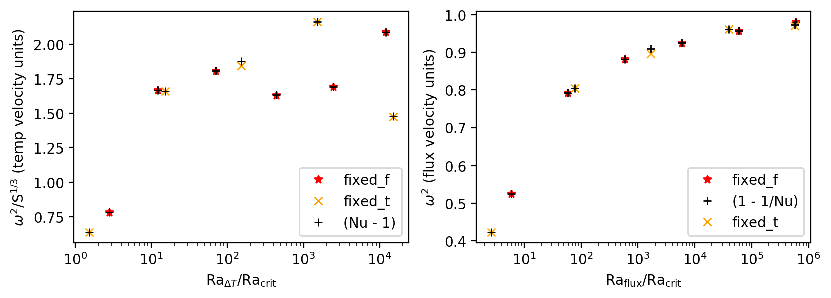
\includegraphics[width=\columnwidth]{figs/unpublished/enstrophy_v_ra.pdf}
    \caption{
	(left) Enstrophy in freefall time units nondimensionalized by the evolved temperature jump across the domain, and normalized by the supercriticality to the third power.
	(right) Enstrophy in freffall time units nondimensionalized by the evolved system flux.
	Simulation measurements are shown from simulations run with fixed flux boundaries (red stars), fixed temperature boundaries (orange crosses), and the expected value of enstrophy as a function of Nu is overplotted.
    \label{fig:enstrophy} }
\end{figure}

\subsection{Where does the enstrophy come from?}
\label{sec:enstrophy_generation}
In order to determine where the enstrophy comes from, we first curl Eqn.~\ref{eqn:momentum} to retrieve the vorticity equation,
\begin{equation}
\pderiv{\bV}{t} = -(\dotp{\bu}{\grad})\bV + (\dotp{\bV}{\grad})\bu + \curl{T_1\hat{z}} + \mR \grad^2 \bV.
\end{equation}
As before, we now dot $\bV$ into this equation and find
\begin{equation}
\pderiv{\omega^2/2}{t} + \Div{\cross{\bV}{\left(T_1\hat{z} - \mR\curl{\bV} + \cross{\bu}{\bV}\right)}} = \dotp{\left(T_1\hat{z} - \mR\curl{\bV} + \cross{\bu}{\bV}\right)}{\curl{\bV}}.
\end{equation}
While generally interesting, we are specifically interested in the 2D case where $\bu = u\hat{x} + w\hat{z}$ and $\bV = \omega\hat{y}$.
In this limit, the enstrophy equation is
\begin{equation}
\pderiv{\omega^2/2}{t} + \Div{\omega\left[\left(T_1 + u\omega - \mR\pderiv{\omega}{x}\right)\hat{x} + \left(w\omega - \mR\pderiv{\omega}{z}\right)\hat{z}\right]} 
= T_1\pderiv{\omega}{x} + \frac{1}{2}\left(w\pderiv{\omega^2}{z} + u\pderiv{\omega^2}{x}\right) - \mR \left(\left[\pderiv{\omega}{z}\right]^2 + \left[\pderiv{\omega}{x}\right]^2\right).
\end{equation}
We can see immediately that all enstrophy fluxes vanish at the boundaries for stress-free boundary conditions.
For this case, we take a volume average and find:
\begin{equation}
\angles{\pderiv{\omega^2}{t}} = 2\angles{T_1\pderiv{\omega}{x}} + \angles{w\pderiv{\omega^2}{z} + u\pderiv{\omega^2}{x}} - 2\mR \angles{\left[\pderiv{\omega}{z}\right]^2 + \left[\pderiv{\omega}{x}\right]^2}.
\end{equation}
There are, on the RHS, three source terms for the enstrophy: one from buoyancy, one from advection, and one from viscosity.
Viscosity acts in a straightforward way: it aims to reduce enstrophy anywhere there is a gradient of the vorticity.
Buoyancy also acts in a fairly straightforward way: Downflows ($T_1 < 0$) separate areas of positive vorticity (on the left) and negative vorticity (on the right), meaning $\pderiv{\omega}{x} < 0$, and the overall productive is positive.
Upflows act in the same way, where the signs on both terms are switched and the product remains positive.
The advective term is more complicated.
The $u \pderiv{\omega^2}{x}$ term seems to destroy enstrophy at plume generation sites and produce it at plume impacting sites.
The $w \pderiv{\omega^2}{z}$ term seems to both generate and destroy enstrophy at  impacting sites (probably canceling out), but it generates enstrophy at plume launching sites.

From some initial simulations, it seems that the buoyant term generates enstrophy and the viscous term destroys it, and that the advective term cancels out due to symmetry in the systems I've studied.

\section{Viscous Heating (and flux in shear flows)}

\section{Internally Heated, Fully Compressible Convection}
\label{sec:internally_heated}

%%%%%%%%%%%%
%%%%%%%%%%%
% Stability and F_avail 
%%%%%%%%%%%
%%%%%%%%%%%%
\subsection{Convective stability and available flux}
\label{sec:stability}
In Boussinesq convection, convective stability is entirely determined by the temperature gradient.
There, negative temperature gradients drive convective motions, and positive temperature gradients are stable.
When compressibility is taken into account, atmospheres can maintain stability even in the presence of a large, negative temperature gradient \cite{spiegel&veronis1960}.
In such atmospheres, it is the gradient of \emph{entropy} which determines stability.
In an ideal gas, the specific entropy gradient is defined
\begin{equation}
\grad S = c_V \grad\ln T - R \grad\ln\rho,
\end{equation}
where $S$, $T$, and $\rho$ are the specific entropy, temperature, and density; $c_V$ is the specfic heat at constant volume; and $R$ is the specific gas constant defining pressure, $P = R \rho T$.
Where stability is concerned, the entropy gradient in compressible systems is a direct analog to the temperature gradient in Boussinesq systems.
Regions with $\grad S < 0$ are unstable to convection, and regions with $\grad S > 0$ are stable.

Assuming that the convective system remains, to first order, in hydrostatic equilibrium, $\grad P = \rho \bm{g}$, the temperature gradient which characterizes a perfectly adiabatic state is:
\begin{equation}
\grad_{\text{ad}} T = \bm{g}/c_P,
\end{equation}
where $\bm{g}$ is the gravity and $c_P$ is the specific heat at constant pressure.
The ``adiabatic temperature gradient,'' $\grad_{\text{ad}} T$, can in general have a large magnitude.
This decreases the simplicity of interpreting the conductive (or radiative) flux in convective systems,
\begin{equation}
\bm{F}_{\text{cond}} = -\kappa \grad T,
\end{equation}
where $\kappa$ is the conductivity.
If a system is driven by some flux, $\bm{F}_{\text{drive}}$, we define the available flux as
\begin{equation}
\bm{F}_{\text{avail}} = \bm{F}_{\text{drive}} - \bm{F}_{\text{ad}},
\end{equation}
where $\bm{F}_{\text{ad}} = -\kappa\grad_{\text{ad}} T$ is the conductive flux carried by the adiabatic temperature gradient.
In regions where the system is being driven with more flux than the adiabatic gradient can carry, $\bm{F}_{\text{avail}} > 0$ and that region of the system is unstable to convection.
Likewise, in stable regions, the system is carrying an amount of flux equal to or less than what can be conducted along the adiabatic temperature gradient, and $\bm{F}_{\text{avail}} \leq 0$.
In this way, $\text{F}_{\text{avail}}$ is a direct analog to the \emph{total} flux carried through a Boussinesq system.

In this work, we will study two systems: polytropic, boundary-driven convection, and convection driven by internal heating and cooling.
Simple polytropic convection is characterized by $\bm{F}_{\text{avail}} = \text{const} > 0$ throughout the domain, and is thus analagous to \RB convection.
Internally heated and cooled convection is characterized by having both regions where $\bm{F}_{\text{avail}}$ is positive and negative.
We expect that accelerated evolution should straightforwardly work in polytropic convection, but that it will require modifications in internally heated convection in order to account for the zero-crossings of $\bm{F}_{\text{avail}}$ in the domain.


%%%%%%%%%%%%
%%%%%%%%%%%
% Atmospheres
%%%%%%%%%%%
%%%%%%%%%%%%
\subsection{Atmospheric models for accelerated evolution}
\label{sec:atmospheres}
In this work, we study convection driven by two different mechanisms in two different atmospheres.
Sample dynamics in disequilibrium states and in relaxed states are shown for both atmospheres in Fig. \ref{fig:atmospheres}.
In the left panels of Fig.~\ref{fig:atmospheres}, the character of boundary-driven convection in a polytropic atmosphere is shown.
In the right panels of Fig.~\ref{fig:atmospheres}, the character of convection driven by a smooth profile of internal heating and cooling is shown.
In all cases, we study a fluid which is a monatomic ideal gas with an adiabatic index of $\gamma = 5/3$ and whose equation of state is $P = R \rho T$, with $P$ the presssure, $\rho$ the density, $T$ the temperature, and $R$ the ideal gas constant.

The initial equilibrium stratification of the polytropic atmospheres is
\begin{equation}
\begin{split}
T_0 = 1 - (z - L_z), \\
\rho_0 = T_0^{m},
\end{split}
\end{equation}
where $z$ is the vertical coordinate, $L_z$ is the atmospheric depth, and the polytropic index is $m = m_{\text{ad}} - \epsilon$, where $m_{\text{ad}} = (\gamma-1)^{-1}$ is the value of $m$ which produces an adiabatic stratification.
Thermodynamics are nondimensionalized so that $P_0 = \rho_0 = T_0 = R = 1$ at the top of the atmosphere, $z = L_z$.
The length scale is nondimensionalized by the temperature gradient length, and thus the nondimensional timescale is the isothermal sound crossing time of this unit length at the top of the atmosphere.
The Mach number of the convective flows scales with $\epsilon$, the superadiabatic excess, like $\text{Ma} \propto \epsilon^{1/2}$.
We studied these atmospheres previously \cite{anders&brown2017}, and found that their dynamics have many similarities to boundary-driven \RB convection, making them a perfect entry point into studying accelerated evolution in stratified domains.

While many computational and experimental studies of convection maintain convective instability through boundary condition specification, this is not generally the case in nature.
Natural convection is generally internally heated -- driven by the gradual deposition of energy.
Internally heated convection can be studied in well-posed Boussinesq systems \cite{goluskin&spiegel2012, goluskin&all2016}, and has even been recently studied in the laboratory \cite{lepot&all2018, bouillaut&all2019}.
In this work, we extend setups similar to these boussinesq studies to the compressible case.

The internally heated and cooled atmospheres are broken up into three different layers: a stable layer at the top of the atmosphere with depth $L_{RT}$, a convective layer with depth $L_C$, and a stable layer at the base of the atmophere with depth $L_{RB}$; the total atmospheric depth is $L_z = L_{RB} + L_C + L_{RT}$.
The initial temperature stratification of these atmospheres is
\begin{equation}
T_0 = 1 - (z - L_z) + \epsilon(A z^3 + B z^2 + Cz + D),
\end{equation}
where $A = \frac{1}{6}$, $B = -\frac{1}{2}(L_{RB} + L_C/2)$, $C = \frac{1}{2}L_{RB}(L_{RB} + L_C)$, and $D = (-AL_z^3 + BL_z^2 + CL_z)$.
This profile maintains thermal equilibrium with an internal heating profile $Q(z) = \kappa \epsilon(z + 2B)$, where $\kappa$, the thermal conductivity, is described shortly.
The density profile is obtained by numerically solving for hydrostatic equilibrium.
Thermodynamics are nondimensionalized in the same manner as in the polytropes.
The length scale is nondimensionalized on the \emph{adiabatic} temperature gradient length scale, $\grad_{\text{ad}} = -g/c_P = -1$, where $g$ is the (uniform) gravity and $c_P$ is the specific heat at constant pressure.
The nondimensional timescale is again the isothermal sound crossing time of that unit length at the top of the atmosphere.

In all atmospheres, the thermal conductivity, $\kappa$ and the dynamic viscosity, $\mu$ are constant in time and uniform in space.
By these choices, the kinematic viscosity, $\nu = \mu/\rho$ and the thermal diffusivity, $\chi = \kappa/\rho$ vary inversely with density.


\section{Stratified Accelerated Evolution}
%%%%%%%%%%%%
%%%%%%%%%%%
% AE METHOD
%%%%%%%%%%%
%%%%%%%%%%%%

\subsection{Modifications to the method of Accelerated Evolution}
\label{sec:ae}
Here we describe extensions of the method of accelerated evolution described in section 3 of \cite{anders&all2018} to compressible systems.
As before, we restrict our study to simulations in which the thermal boundary conditions specify the flux at the lower boundary, $F_{\text{bot}}$, and the temperature at the top boundary, $T_{\text{top}}$.
We additionally restrict this study to the case in which the thermal conductivity, $\kappa$, is constant.
Assuming that the initial atmospheric state (which will be denoted by subscript ``0'') is in thermal equilibrium, the conductive flux can be broken up into two pieces:
\begin{equation}
F_{\text{cond}} = -\kappa\partial_z T_0 = \kappa \frac{g}{c_P} + F_{\text{avail}},
\end{equation}
where $T_0$ is the initial temperature profile, $g$ is the gravitational acceleration, and $c_P$ is the specific heat at constant pressure.
Here, we have split the flux into a component carried by the adiabatic temperature gradient, $\partial_z T_{\text{ad}} = -g/c_p$, and the flux in excess of that, $F_{\text{avail}}$.
As a quantity of flux equal to $-\kappa\partial_z T_{\text{ad}}$ can be carried stably, only the flux in excess of the adiabatic flux is available for the convection to carry, and we therefore refer to it as the ``available flux,'' $F_{\text{avail}}$.

In \RB convection, flux is entirely carried by a combination of the convective enthalpy flux and the conductive flux.
In stratified systems, convection carries energy not only through enthalpy fluxes, but also through fluxes of potential energy, kinetic energy, and viscous forces.
All of these new fluxes are driven by convection, and we therefore define the convective flux,
\begin{equation}
\bm{F}_{\text{conv}} \equiv \bm{F}_{\text{enth}} + \bm{F}_{\text{KE}} + \bm{F}_{\text{PE}} + \bm{F}_{\text{visc}},
\end{equation}
where $\bm{F}_{\text{enth}} \equiv \rho\bm{u}(c_V T + P/\rho)$ is the enthalpy flux, $\bm{F}_{\text{KE}} \equiv \rho|\bm{u}|^2\bm{u}/2$ is the kinetic energy flux, $\bm{F}_{\text{PE}} \equiv \rho\bm{u}\phi$ (with $\phi \equiv -gz$) is the potential energy flux, and $\bm{F}_{\text{visc}} \equiv -\rho\nu\bm{u}\cdot\lilstressT$ is the viscous flux.
Here, $\bm{u}$ is the velocity, $c_V$ is the specific heat and constant volume, $P$ is the pressure, $\phi$ is the gravitational potential, $\nu$ is the kinematic viscosity, and $\lilstressT$ is the viscous stress tensor in units of inverse time.
The total relevant superadiabatic flux through such a system is thus $F_{\text{superad}} \equiv F_{\text{conv}} + F_{\text{cond,s}}$, where the superadiabatic portion of the conductive flux is $F_{\text{cond,s}} = -\kappa(\partial_z (T_0 + T_1) - \partial_z T_{\text{ad}})$.

As in \cite{anders&all2018}, we find that the fluxes carried through these systems at early times can exceed $F_{\text{avail}}$ as the system leaks out its energy and approaches its relaxed states.
As a result, we define the profile,
\begin{equation}
\xi_{\text{BD}}(z, t) = \frac{F_{\text{avail}}}{F_{\text{superad}}},
\label{eqn:xi_BD}
\end{equation}
which has a value of unity where the system is carrying the expected amount of flux, but whose value is generally less than one at these early times.
Here, $\xi$ is a measure of the factor by which the flux through the system must be reduced in order for the system to reach its final, equilibrium state.
In boundary-driven convection, where $F_{\text{avail}}$ is a uniform, positive value throughout the whole domain, this definition of $\xi$ is fairly robust.

Unfortunately, in convectively stable regions, the value of $F_{\text{avail}}$ is definitionally negative.
In such regions, the adiabatic gradient is capable of carrying more flux than it is currently carrying.
As a result, in convective domains in which stable layers and unstable layers bound one another, the profile of $F_{\text{avail}}$, and thus $F_{\text{superad}}$, experiences zero-crossings, and at those locations, Eqn.~\ref{eqn:xi_BD} is undefined.
A more general profile can be defined,
\begin{equation}
\xi_{\text{SL}} = \frac{F_{\text{avail} + \tilde{F}}}{F_{\text{superad} + \tilde{F}}},
\end{equation}
where $\tilde{F}$ is a flux offset that ensures that both the numerator and denominator are positive-definite.
While $\xi_{\text{SL}}$ avoids the pathologies of $\xi_{\text{BD}}$ near zero-crossings, if $\tilde{F}$ and $F_{\text{avail}}$ are approximately the same order of magnitude, $\xi_{\text{SL}}$ no longer accurately describes the factor by which the flux through the system needs to be reduced to achieve an equilibrated, relaxed state.
We find that generally $F_{\text{avail}} \approx F_{\text{superad}}$ in the stable regions studied in this work, and so there $\xi_{\text{BD}} \approx \xi_{\text{SL}} \approx 1$.
This means that the discrepancies between the two profiles exist in the convective region.
In order to account for these differences without affecting the stable regions, we define:
\begin{equation}
\xi = S (\xi_{\text{SL}} - 1) + 1,
\label{eqn:xi_stable}
\end{equation}
where 
$$
S \equiv \text{median}\left(\frac{\xi_{\text{BD}}(z) - 1}{\xi_{\text{SL}}(z) - 1}\right), \forall z \in F_{\text{superad}}(z) > \frac{1}{4}\text{max}(F_{\text{superad}}).
$$

For our boundary driven convection, we define $\xi \equiv \xi_{\text{BD}}$, but for all simulations which include a stable layer, we define $\xi$ as in Eqn.~\ref{eqn:xi_stable}.

With this definition of $\xi$, we solve the boundary value problem,
%\begin{gather}
%\partial_z M_1 = \rho_0(e^{\ln\rho_1} - 1), \\
%\kappa\partial_z^2 T_1 = \partial_z(\xi \angles{F_{\text{conv}}}), \\
%\partial_z(T_1) + T_1 \partial_z(\ln\rho_0) + T_0\partial_z(\ln\rho_1) = -T_1\partial_z(\ln\rho_1) - \bar{\xi}^{\frac{2}{3}}\angles{\bm{u}\cdot\grad w}.
%\end{gather}
with the boundary conditions $M_1 = 0$ at $z = [0, L_z]$, $\partial_z T_1 = 0$ at $z = 0$, and $T_1 = 0$ at $z = L_z$.



\section{An $\epsilon$ nondimensionalization of the Fully Compressible Equations}
\subsection{The fully compressible equations}
We define the fully compressible equations in \citet{anders&brown2017} as:
\begin{gather}
\partial_{\td{t}} \td{\ln \rho_1} + \td{\uvec}\cdot\td{\grad} \td{\ln\rho_0} + \td{\grad}\cdot\td{\uvec} = -\td{\uvec}\cdot\td{\grad}\td{\ln\rho_1} 
\label{eqn:unscaled_continuity}
\\
\begin{split}
\partial_{\td{t}} \td{\uvec} + R(\td{\grad} \td{T_1} + \td{T_1} \td{\grad}\td{\ln\rho_0} + \td{T_0} \td{\grad}\td{\ln\rho_1})
- \td{\nu}\left(\td{\grad}^2 \td{\uvec} + \frac{1}{3}\td{\grad}(\td{\grad}\cdot\td{\uvec}) + \td{\grad}\td{\ln\rho_0}\cdot\td{\lilstressT}\right)
- \td{\grad}\td{\nu}\cdot\td{\lilstressT}
\\= -\td{\uvec}\cdot\td{\grad}\td{\uvec} - R\td{T_1}\td{\grad}\td{\ln\rho_1} + \td{\nu}\td{\grad}\td{\ln\rho_1}\cdot\td{\lilstressT}
\end{split}
\label{eqn:unscaled_momentum}
\\
\begin{split}
\partial_{\td{t}} \td{T_1} + \td{\uvec}\cdot\td{\grad} \td{T_0} + \td{T_0}(\gamma-1)\td{\grad}\cdot\td{\uvec} 
- \frac{1}{c_V}\left(\td{\chi}\left\{\td{\grad}^2 \td{T_1} + \td{\grad}\td{\ln\rho_0} \cdot\td{\grad} \td{T_1} + \td{\grad}\td{\ln\rho_1}\cdot\td{\grad} \td{T_0}\right\} 
+ \td{\grad}\td{\chi}\cdot\td{\grad} \td{T_1}\right)
\\= \frac{\td{\chi}}{c_V}\td{\grad}\td{\ln\rho_1}\cdot\td{\grad} \td{T_1} - \td{\uvec}\cdot\td{\grad} \td{T_1} - \td{T_1}(\gamma-1)\td{\grad}\cdot\td{\uvec}
+ \frac{\td{\nu}}{c_V}\td{\lilstressT}\cdot\td{\grad}\cdot\td{\uvec}.
\end{split}
\label{eqn:unscaled_energy}
\end{gather}
Here, the tildes over the terms stand for ``dimensionful" quantities (or quantities that I haven't
rescaled yet). Those are going to be dropped. Only two real assumptions have happened so far:
I've assumed hydrostatic equilibrium of the background quantities in the momentum equation,
and I've assumed thermal equilibrium of the background quantities in the energy equation.
We now rescale the equations such that
\begin{equation}
\begin{split}
\td{T_0} =  T_0, 		\qquad &\td{\ln\rho_0} = \ln\rho_0\qquad, \\
\td{T_1} = \epsilon T_1, \qquad &\td{\ln\rho_1} = \epsilon\ln\rho_1, \\
\td{\grad} = L^{-1}\grad,  		\qquad &\partial_{\td{t}} = \tau^{-1}\partial_t, \\
\td{\nu} = \nu\xi(z),				\qquad &\td{\chi} = \chi\xi(z),\\
v_{\ff} = L/\tau, \qquad &%\td{c_V} = R c_V,
\end{split}
\end{equation}
Under these rescalings we retrieve the equations:
\begin{gather}
\partial_t \ln\rho_1 + \epsilon^{-1}\left(\uvec\cdot\grad\ln\rho_0 + \DivU\right)
= -\uvec\cdot\ln\rho_1
\\
\begin{split}
\partial_t \uvec + \frac{R\epsilon}{v_{\ff}^2}\left(\grad T_1 + T_1\grad\ln\rho_0 + T_0\grad\ln\rho_1\right)
- \frac{\nu\tau}{L^2}\left( \xi\left[\grad^2\uvec + \frac{1}{3}\grad(\DivU) + \grad\ln\rho_0\cdot\lilstressT\right] + \grad\xi\cdot\lilstressT\right)
\\ = - \uvec\cdot\grad\uvec - \frac{R\epsilon^2}{v_{\ff}^2}T_1\grad\ln\rho_1
+ \frac{\nu\epsilon\tau}{L^2}\xi\grad\ln\rho_1\cdot\lilstressT
\end{split}
\\
\begin{split}
\partial_t T_1 + \epsilon^{-1}\left(\uvec\cdot\grad T_0 + T_0(\gamma-1)\DivU\right)
-\frac{\chi \tau}{c_V L^2}\left(\xi\left[\grad^2 T_1 + \grad\ln\rho_0\cdot\grad T_1 + \grad\ln\rho_1 \cdot\grad T_0 \right] + \grad\xi\cdot\grad T_1\right)
\\= \frac{\epsilon\chi\tau}{c_V L^2}\xi\grad\ln\rho_1 \cdot\grad T_1 - 
\left(\uvec\cdot\grad T_1 + T_1(\gamma-1)\DivU\right) + \frac{\nu}{c_V \epsilon \tau }\xi\lilstressT\cdot\grad\cdot\uvec.
\end{split}
\end{gather}
Making the following assumption and defining the following non-dimensional quantities,
\begin{equation}
v_{\ff}^2 = \epsilon, \qquad \tRe_{\ff} = \frac{v_{\ff} L}{\nu}, \qquad
\tPe_{\ff} = \frac{v_{\ff} L}{\chi}, \qquad \tRe_{\ff} = \tPr \tPe_{\ff},
\end{equation}
We arrive at the rescaled FC equations
\begin{gather}
\partial_t \ln\rho_1 + \epsilon^{-1}\left(\uvec\cdot\grad\ln\rho_0 + \DivU\right)
= -\uvec\cdot\ln\rho_1
\\
\begin{split}
\partial_t \uvec + R(\grad T_1 + T_1\grad\ln\rho_0 + T_0\grad\ln\rho_1)
- \frac{1}{\tRe_\ff}\left( \xi\left[\grad^2\uvec + \frac{1}{3}\grad(\DivU) + \grad\ln\rho_0\cdot\lilstressT\right] + \grad\xi\cdot\lilstressT\right)
\\ = - \uvec\cdot\grad\uvec - \epsilon R T_1\grad\ln\rho_1
+ \frac{\epsilon}{\tRe_\ff}\xi\grad\ln\rho_1\cdot\lilstressT
\end{split}
\\
\begin{split}
\partial_t T_1 + \epsilon^{-1}\left(\uvec\cdot\grad T_0 + T_0(\gamma-1)\DivU\right)
-\frac{1}{c_V \tPe_\ff}\left(\xi\left[\grad^2 T_1 + \grad\ln\rho_0\cdot\grad T_1 + \grad\ln\rho_1 \cdot\grad T_0 \right] + \grad\xi\cdot\grad T_1\right)
\\= \frac{\epsilon}{c_V  \tPe_\ff} \xi\grad\ln\rho_1 \cdot\grad T_1 - 
\left(\uvec\cdot\grad T_1 + T_1(\gamma-1)\DivU\right) + \frac{1}{c_V \tRe_\ff}\xi\lilstressT\cdot\grad\cdot\uvec.
\end{split}
\end{gather}

At this point, all that's left to do is choose either a non-dimensional length scale (from which
time is chosen), or vice-versa. This choice will probably differ based on the problem you're
studying, but some rough ideas would be:
\begin{enumerate}
\item (convection) $L$ is the domain depth
\item (thermals)   $L$ is the diameter of the thermal
\item (acoustic excitation) $L$ is the width of the plume / cold source.
\end{enumerate}
The temperature gradient would need to be scaled by this length scale appropriately, and the 
temperature profile (and probably all the thermo profiles?) would need to be scaled appropriately
by $\bar{T}$ for the choice of $\epsilon$ used.



\section{Convection with Kramer's Opacity}
\subsection{The Experiment -- Single Layer atmosphere}
Our initial conditions are an adiabatic polytrope,
$$
T = L_z + 1 - z \qquad \rho = T^{m_{ad}},
$$
where $L_z = np.exp(m_{ad}/n_rho) - 1$ is the depth, $z = [0, L_z]$, and
$m_{ad} = (\gamma - 1)^{-1}$.
The opacity is a Kramer's opacity \cite{kapyla&all2017} such that the
radiative conductivity is
$$
\kappa(z) = \kappa_0 \left(\frac{\rho}{\rho_c}\right)^{-(1+a)} \left(\frac{T}{T_c}\right)^{(3-b)},
$$
where $a = 1$, $b = -7/2$, and the thermal diffusivity is 
$\chi = \kappa / (\rho c_P)$. In general, for a polytropic
atmosphere, $\rho \propto T^m$, there is a polytropic index
that achieves a constant Kramer's opacity \cite{jones1976}
$$
m_{kram} = \frac{3 - b}{1 + a}.
$$
We hypothesize that, in general, if $m_{kram}$ differs from
$m_{ad}$ by O($\epsilon$), then the initially adiabatic atmosphere will
drive convective motions like the $\epsilon$ parameter we published
previously \cite{anders&brown2017}. In this work, we will fix
$a = 1$, and study $b = (0, -3.5]$, from very small $b = -10^{-4}$,
up to $b = -1$ and $b = -3.5$, the true value of $b$ for free-free
interactions, deep in the Sun. For our choice of $a = 1$,
\begin{equation}
m_{kram} = 1.5 - b/2 = m_{ad} - b/2.
\end{equation}
So $b$ will be one of our control parameters in our experiment. In
general, for our polytropic initial conditions, and with a radiative
flux of $F = -\kappa_0 \rho^{-(1+a)}T^{(3-b)} \grad T$,
\begin{equation}
\frac{F_{top}}{F_{bot}} = \frac{-\kappa_0\cdot 1 \cdot 1 \cdot -1}
                         {-\kappa_0\cdot e^{-(1+a)n_\rho} (L_z+1)^{(3-b)}\cdot -1}
= e^{(1+a)n_\rho - (3-b)n_\rho / m_{ad}}
\end{equation}
Assuming that the amount of the flux that needs to be carried at the top of
the atmosphere is proportional to the size of entropy perturbations that
carry the flux, and that the flux at the
bottom is the fixed flux that must be transported through the atmosphere, 
then I assume that the characteristic entropy perturbations are of the order
$$
|S| \sim \bigg| 1 - e^{(1+a)n_\rho - (3-b)n_\rho / m_{ad}} \bigg| = \bigg| 1 - e^{b n_\rho / m_{ad}} \bigg|,
$$
and when $b$ is small, $e^{b n_\rho / m_{ad}} = 1 + b n_\rho / m_{ad}$, and
$|S| ~ b n_\rho / m_{ad}$.

We will also define a Rayleigh number,
\begin{equation}
\text{Ra} = \frac{g L_z^3 |S|/c_P}{\nu_t \chi_t},
\end{equation}
which will determine
$$
\kappa_0 = \frac{\chi_t c_P}{e^{n_\rho(-(1+a) + (3-b)/m_{ad}}}
$$
We also set $T_c$ and $\rho_c$ to be the values of $T$ and $\rho$ at the
bottom of the atmosphere, $T_c = L_z + 1$, $\rho_c = e^{n_\rho}$, such that
$\kappa = \kappa_0$ at the bottom of the atmosphere, and thus $\kappa_0$ directly
controls the flux through the system. In order to study systems with comprehensible
prandtl numbers, we set
$$
\mu = \text{Pr}\cdot\kappa(\rho_0, T_0)/c_P,
$$
where Pr $\equiv \nu/\chi$. This keeps a constant Pr with depth in the intial state,
although with $\mu$ fixed, Pr is allowed to evolve.

So under the specification of Pr, Ra, $b$, and $n_\rho$, our convective system
is fully specified, as far as I can tell.

The characteristic convective timescale is still the buoyancy time,
$$
t_b = \sqrt{\frac{L_z}{g (|S|/c_P)}}.
$$




\subsection{Implementation of Kramer's Opacity in Dedalus (easier)}
After talking with Ben, I realize that the implementation I have below in
the next section is harder than it needs to be. Let's look at this a different way.
If we have a radiative conductivity of the form,
\begin{equation}
\kappa(z) = \kappa_0 \rho^{-(1 + a)} T^{3 - b},
\end{equation}
then we can taylor expand this conductivity into its constant, linear, and
nonlinear components,
\begin{equation}
\kappa(\rho, T) = \kappa(\rho_0, T_0) 
+ \frac{\partial \kappa}{\partial T}\bigg|_{\rho_0, T_0}(T - T_0)
+ \frac{\partial \kappa}{\partial \ln\rho}\bigg|_{\rho_0, T_0}(\ln\rho - \ln\rho_0)
+ \kappa_{\text{NL}}.
\end{equation}
To evaluate that, we need a couple of derivatives:
\begin{equation}
\begin{split}
&\frac{\partial \kappa}{\partial T}\bigg|_{\rho_0, T_0} = 
\kappa_0(3-b)\rho_0^{-(1+a)}T_0^{2-b} = (3-b)\frac{\kappa(\rho_0, T_0)}{T_0} \\
&\frac{\partial \kappa}{\partial \ln\rho}\bigg|_{\rho_0, T_0} =
\rho\frac{\partial \kappa}{\partial \rho}\bigg|_{\rho_0, T_0} =
-(1+a)\kappa_0 \rho_0^{-(1+a)} T_0^{3-b} = -(1+a)\kappa(\rho_0, T_0),
\end{split}
\end{equation}
and after quick substitions,
\begin{equation}
\kappa(\rho, T) = \kappa(\rho_0, T_0)\left( 1 +
(3 - b)\frac{T_1}{T_0} - (1 + a) \ln\rho_1 \right)
+ \kappa_{\text{NL}}
\end{equation}
At this point, I will define the constant, linear, and nonlinear parts of $\kappa$,
\begin{equation}
\begin{split}
&\kappa_\text{C} \equiv \kappa(\rho_0, T_0) \\
&\kappa_\text{L} \equiv \kappa_C\left(
(3 - b)\frac{T_1}{T_0} - (1 + a) \ln\rho_1 \right) \\
&\kappa_{\text{NL}} \equiv \kappa - \kappa_\text{C} - \kappa_{\text{L}}.
\end{split}
\end{equation}

On the LHS of the energy equation, we have a term
\begin{equation}
\text{DivFcond} = \Div{-\kappa\grad T} 
= -(\kappa\grad^2 T + \grad \kappa\cdot\grad T)
\end{equation}
This can be simply broken up into linear and nonlinear components,
\begin{equation}
\begin{split}
&\text{DivFcond\_L} = -\left(\kappa_\text{L}\grad^2 T_0 
+ \kappa_\text{C} \grad^2 T_1 
+ \grad T_0 \cdot \grad \kappa_\text{L}
+ \grad T_1 \cdot \grad \kappa_\text{C}\right) \\
&\text{DivFcond\_NL} = -\left(
(\kappa - \kappa_\text{L})\grad^2 T_0
+ (\kappa - \kappa_\text{C})\grad^2 T_1
+ \grad T_0 \cdot \grad(\kappa - \kappa_\text{L}) 
+ \grad T_1 \cdot \grad(\kappa - \kappa_\text{C}) \right)
\end{split}
\end{equation}

\subsection{Difficulties}








\section{Turbulent Thermals}





